\section{Installation}
\label{sec:Installation}
In diesem Kapitel wird die Vorgehensweise erläutert, um die \gls{app} Fast 
Diagnose mit einer ABB-Steuerung nutzen zu können. Für das Einspielen der 
entsprechenden Dateien wird Robotstudio 5.61 verwendet. Das gesamte ABB-System 
ist unter folgendem Link verfügbar: \url{https://github.com/MRixen/Doku_App/}.

Folgende Komponenten müssen in das bestehende ABB-Projekt 
integriert werden:
\begin{itemize}
\item Task ServerComm mit Modul ServerComm (s. \ref{fig:taskServerComm})
\begin{figure}[H]
	\centering
	\fbox{	
	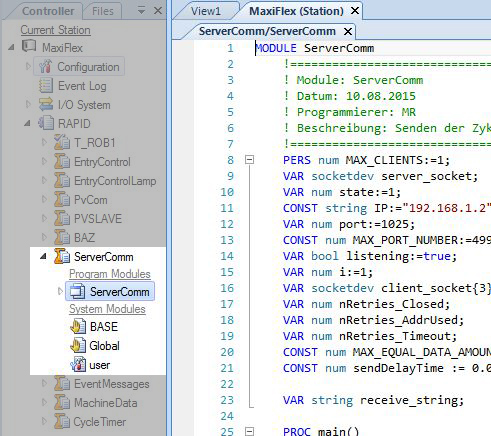
\includegraphics[width=0.6\textwidth]{03_Grafiken/taskServerComm.jpg}}
	\caption[Task und Modul ServerComm]{Task und Modul ServerComm}
	\label{fig:taskServerComm}
\end{figure}
\item Task und Modul EventMessages (s. \ref{fig:taskEventMessages})
\begin{figure}[H]
	\centering
	\fbox{	
	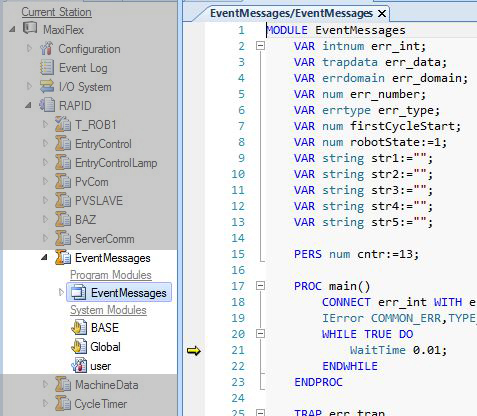
\includegraphics[width=0.6\textwidth]{03_Grafiken/taskEventMessages.jpg}}
	\caption[Task und Modul EventMessages]{Task und Modul EventMessages}
	\label{fig:taskEventMessages}
	\end{figure}
\item Task und Modul MachineData (s. \ref{fig:taskMachineData})
	\begin{figure}[H]
		\centering
		\fbox{	
		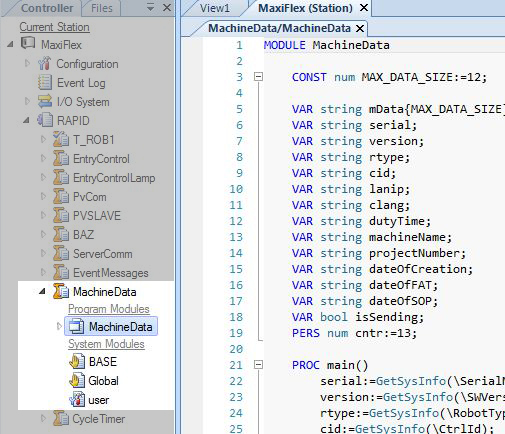
\includegraphics[width=0.6\textwidth]{03_Grafiken/taskMachineData.jpg}}
		\caption[Task und Modul MachineData]{Task und Modul MachineData}
		\label{fig:taskMachineData}
		\end{figure}
\item Task und Modul EventMessages (s. \ref{fig:taskCycleTimer})
\begin{figure}[H]
	\centering
	\fbox{	
	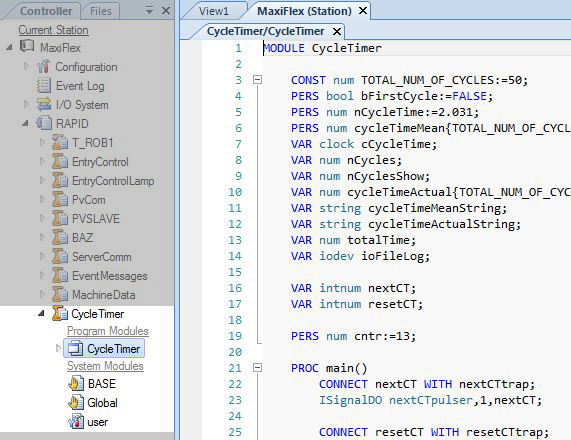
\includegraphics[width=0.6\textwidth]{03_Grafiken/taskCycleTimer.jpg}}
	\caption[Task und Modul CycleTimer]{Task und Modul CycleTimer}
	\label{fig:taskCycleTimer}
\end{figure}

\end{itemize}  
Folgende Komponenten müssen in dem bestehenden ABB-Projekt 
ergänzt/modifiziert werden:
\begin{itemize}
\item Automatik loading of Modules (s. \ref{fig:autoLoad})
\begin{figure}[H]
	\centering
	\fbox{	
	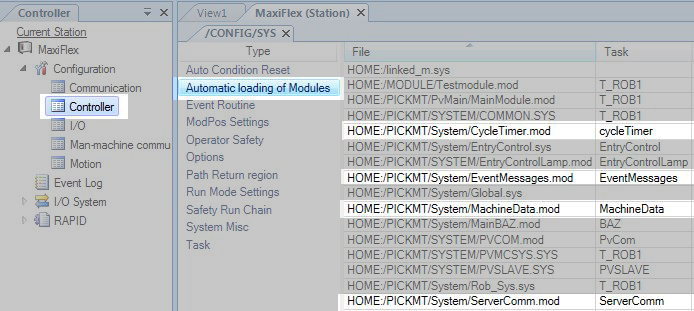
\includegraphics[width=0.6\textwidth]{03_Grafiken/autoLoad.jpg}}
	\caption[Automatic loading]{Automatic loading}
	\label{fig:autoLoad}
\end{figure}
\item I/Os (s. \ref{fig:signale})
\begin{figure}[H]
	\centering
	\fbox{	
	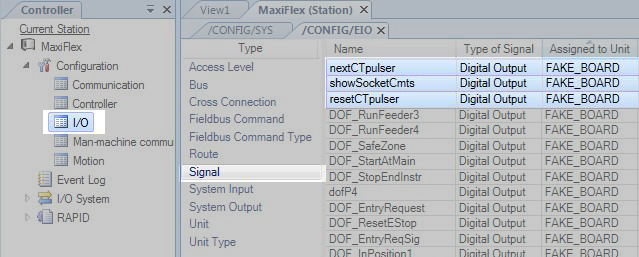
\includegraphics[width=0.6\textwidth]{03_Grafiken/signals.jpg}}
	\caption[Signale hinzufügen]{Signale hinzufügen}
	\label{fig:signale}
	\end{figure}
\item Modifikation von Global.sys
\begin{figure}[H]
	\centering
	\fbox{	
	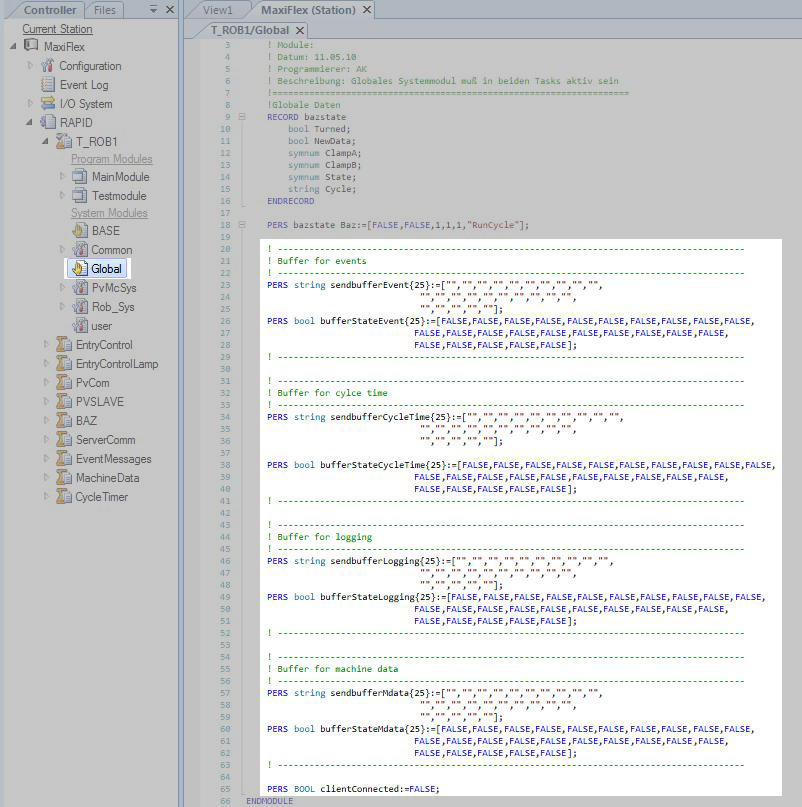
\includegraphics[width=1\textwidth]{03_Grafiken/globalSys.jpg}}
	\caption[Global.sys]{Global.sys}
	\label{fig:globalSys}
\end{figure}
Die Buffer, sowie die Variable \textit{clientConnected} müssen global für jede 
Task verfügbar sein.
\end{itemize}  
